\section{Gangbild Anpassungen}
Das natürlich erlernte Gangbild eines gesunden Menschen ist sehr komplex. Im folgenden Kapitel wird das Gangbild des Mixamo Charakters basierend auf den Gangphasen der Menschlichen Fortbewegung analysiert und angepasst. Wie bereits in der Analyse der Walker Demo erwähnt, ist das Gangbild des Walker Demo Läufers menschenähnlich und für die vereinfachte Darstellung des Charakters durchaus ausreichen. Die gesteigerte Komplexität des 3D Modells beim Mixamo Charakter führt bei der Wahrnehmung einem gesteigerten Realismus. Der Mixamo Charakter lernt zudem mehr ein galoppieren als das laufen welches der Walker Demo Läufer nach dem Training aufweist. Durch den gesteigerten Realismus und die Verschlechterung des Gangbilds wird in folgendem Kapitel getestet wie zusätzliche Belohnungen das erlernte Gangbild beeinflussen können.

\subsection{Belohnung für Beinwechsel}
Das Menschliche Gangbild besteht aus sich wiederholenden Phasen, die abwechselnd bei beiden Beinen durchlaufen werden. Um den Läufer dazu zu motivieren in einem regelmäßigen Intervall das vorangehende Bein zu wechseln wird ein Timer eingeführt welcher von 0 startet sobald das vorderste Bein in Zielrichtung gewechselt wurde. Ausgehend der verstrichenen Zeit seit dem letzten Wechsel bekommt der Läufer dann eine Strafe. Wie in Abbildung \ref{fig:plot_beinwechsel} zu sehen ist Bestrafung bis 1,2 Sekunden 0. Bleibt ein Bein länger als 1,2 Sekunden vorne steigt die Bestrafung linear an bis sie bei 5,2 Sekunden das Maximum von -1 erreicht.\cite{aiwarehouse}

\begin{figure}[H]
  \centering
  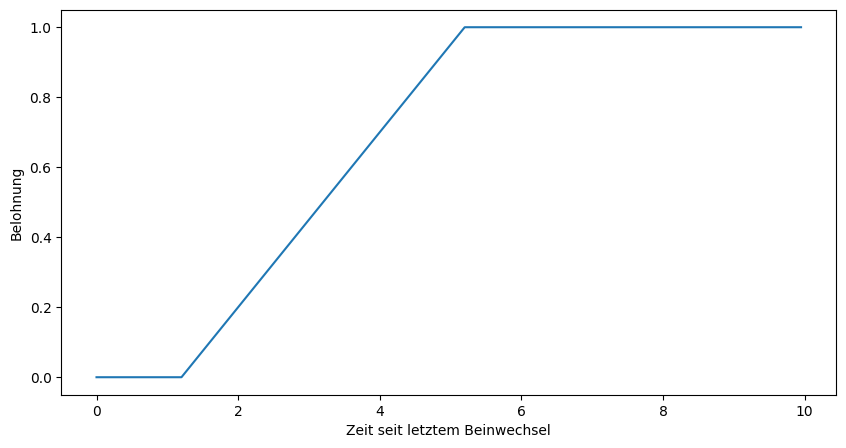
\includegraphics[width=0.9\textwidth]{img/plot_beinwechsel} 
  \caption{Beinwechsel Belohnung}
  \label{fig:plot_beinwechsel}
\end{figure}

Das einführen dieser Bestrafung hat beim Training erfolgreich dazu geführt das der Läufer in regelmäßigen Abständen das Standbein wechselt und somit ein natürlicheres Gangbild entwickelt (siehe Abbildung \ref{fig:mixamo_versuch11_gangbild}).

\begin{figure}[H]
  \centering
  \begin{tabular}{ccc}
    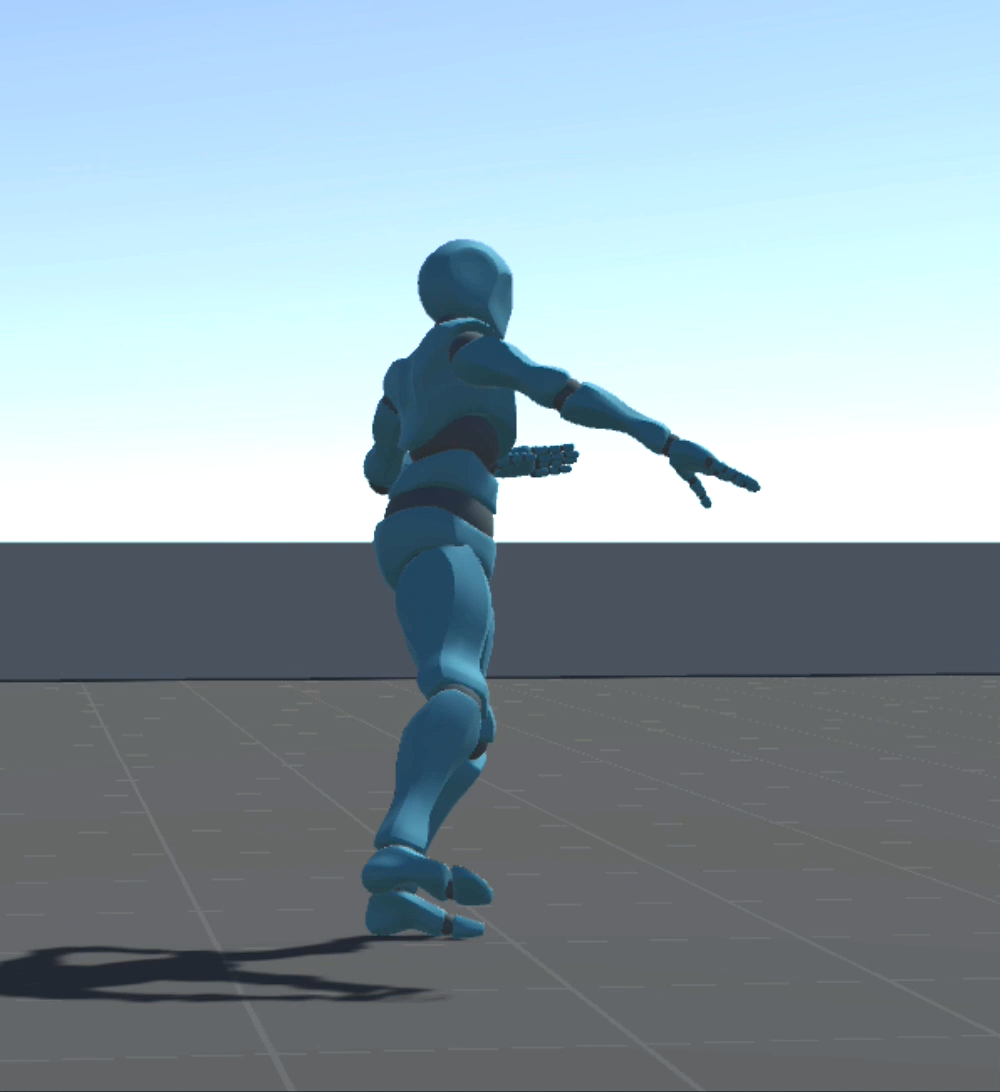
\includegraphics[width=0.27\textwidth]{img/charakter_mixamo_laufen1} & 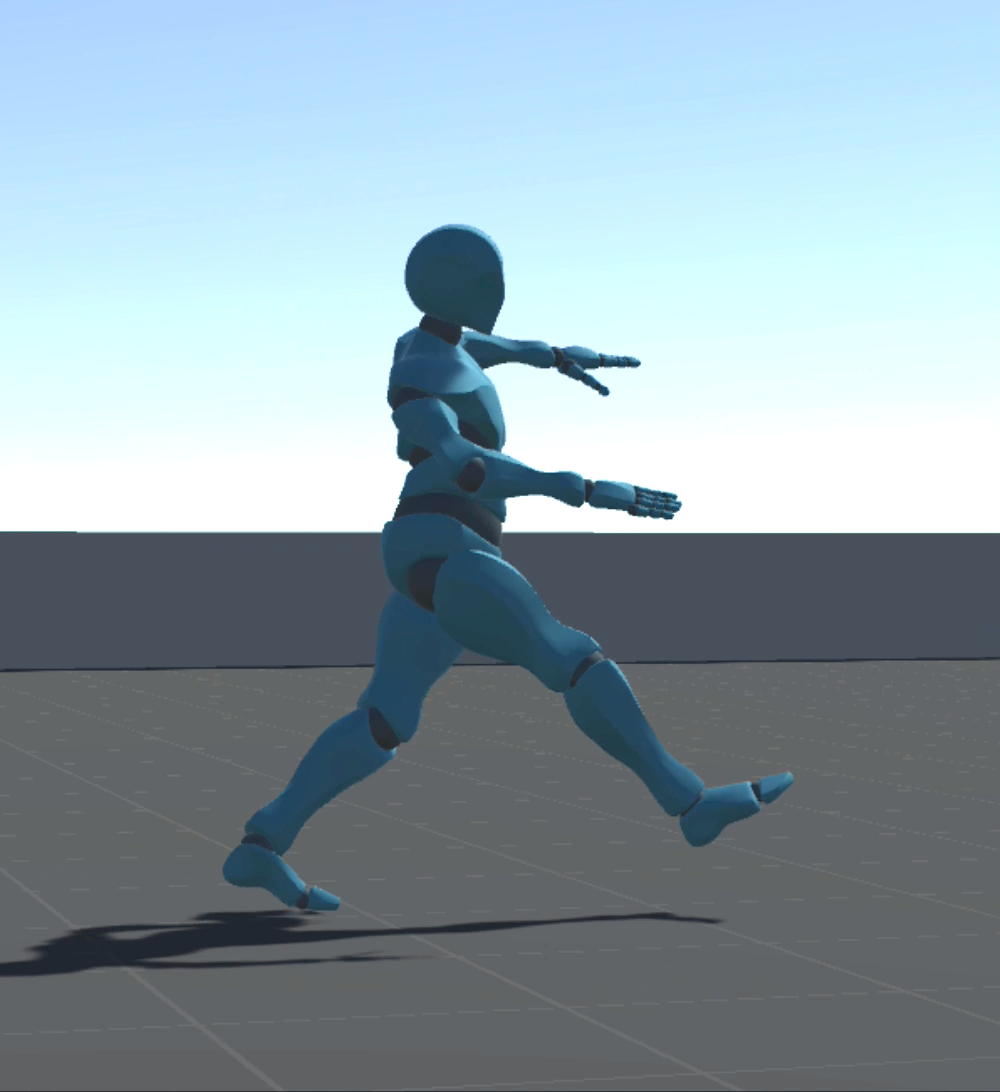
\includegraphics[width=0.27\textwidth]{img/charakter_mixamo_laufen2}  & 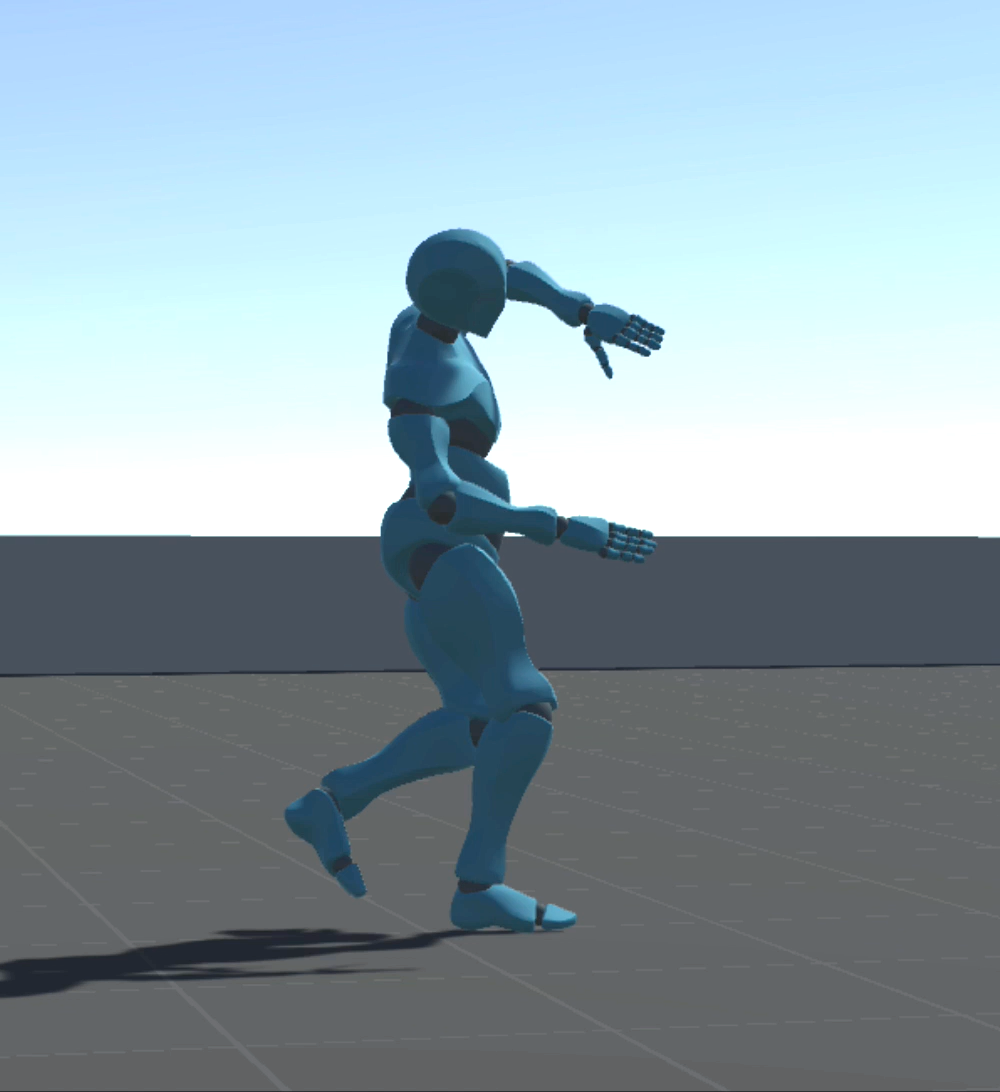
\includegraphics[width=0.27\textwidth]{img/charakter_mixamo_laufen3} \\
    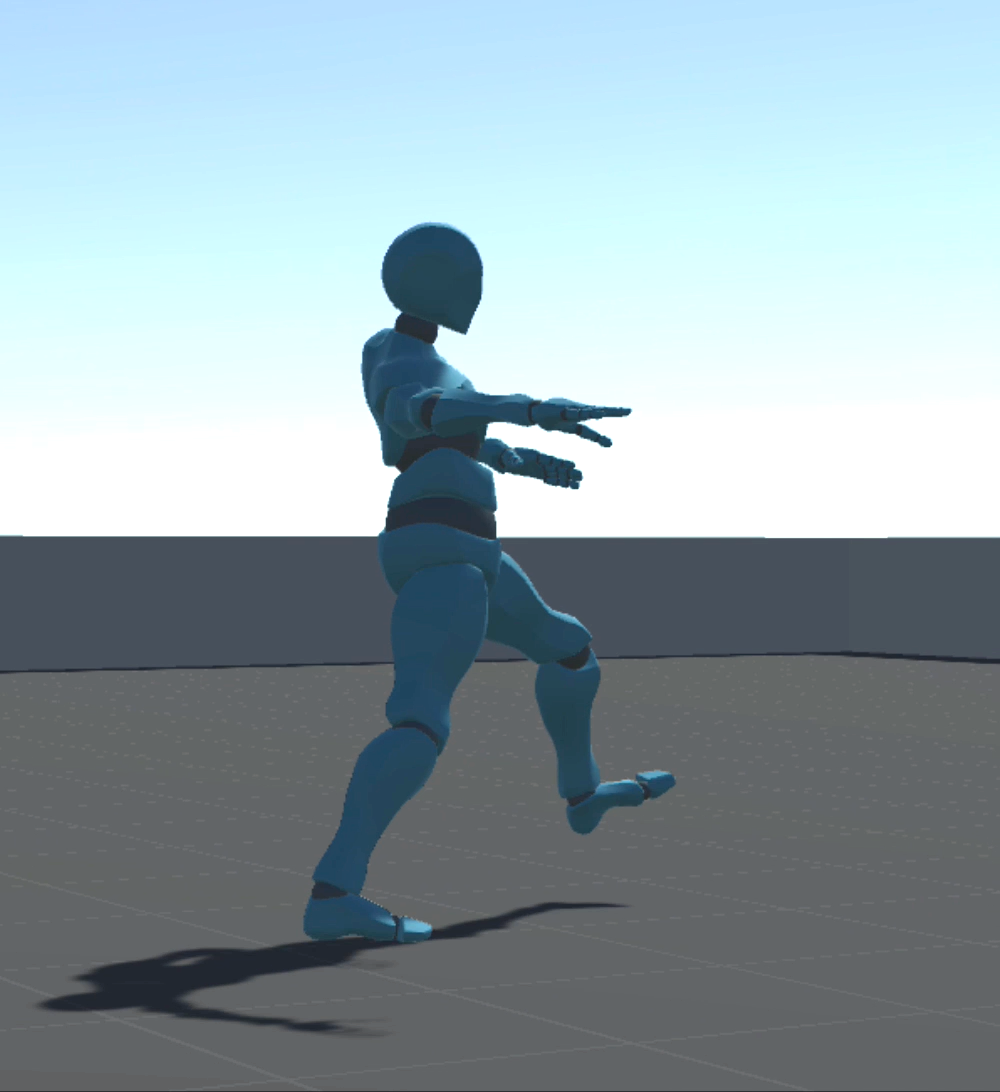
\includegraphics[width=0.27\textwidth]{img/charakter_mixamo_laufen4}  & 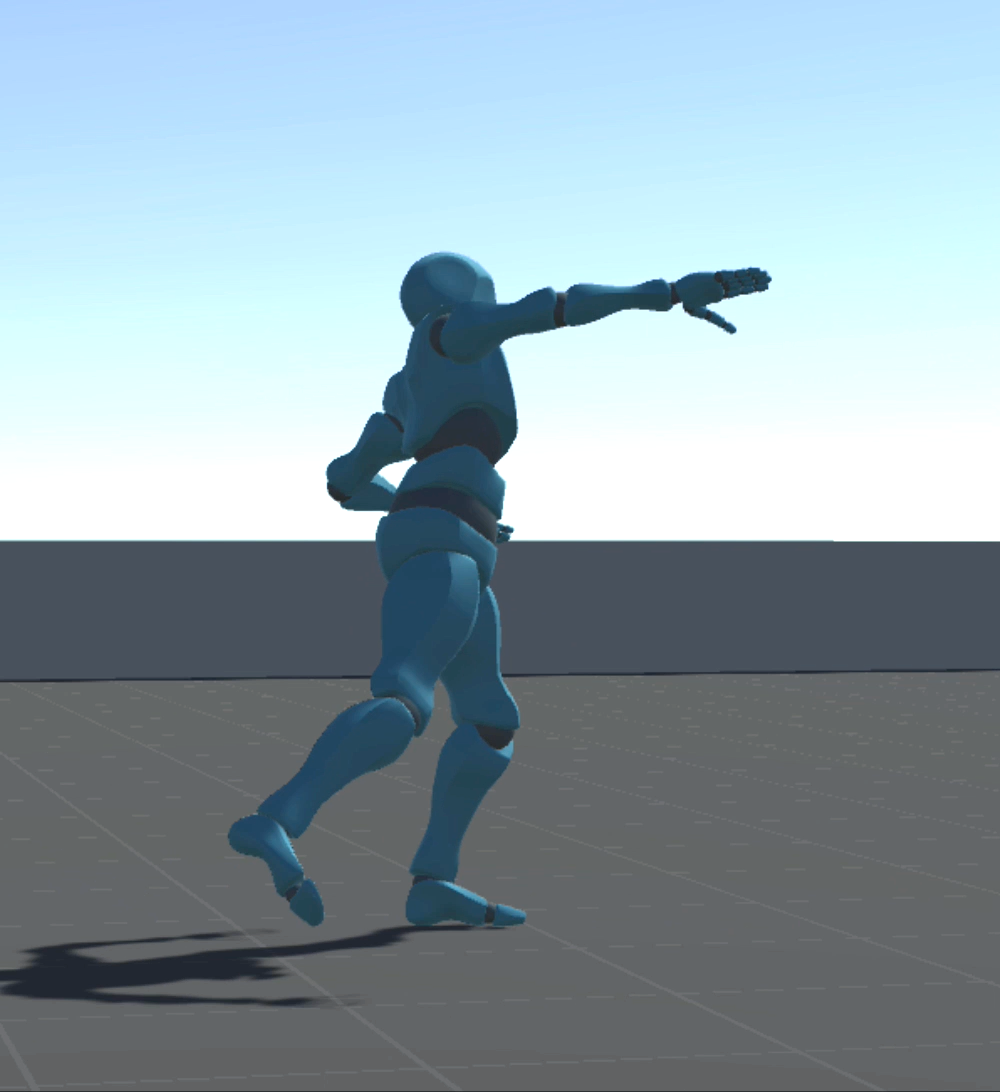
\includegraphics[width=0.27\textwidth]{img/charakter_mixamo_laufen5}  & 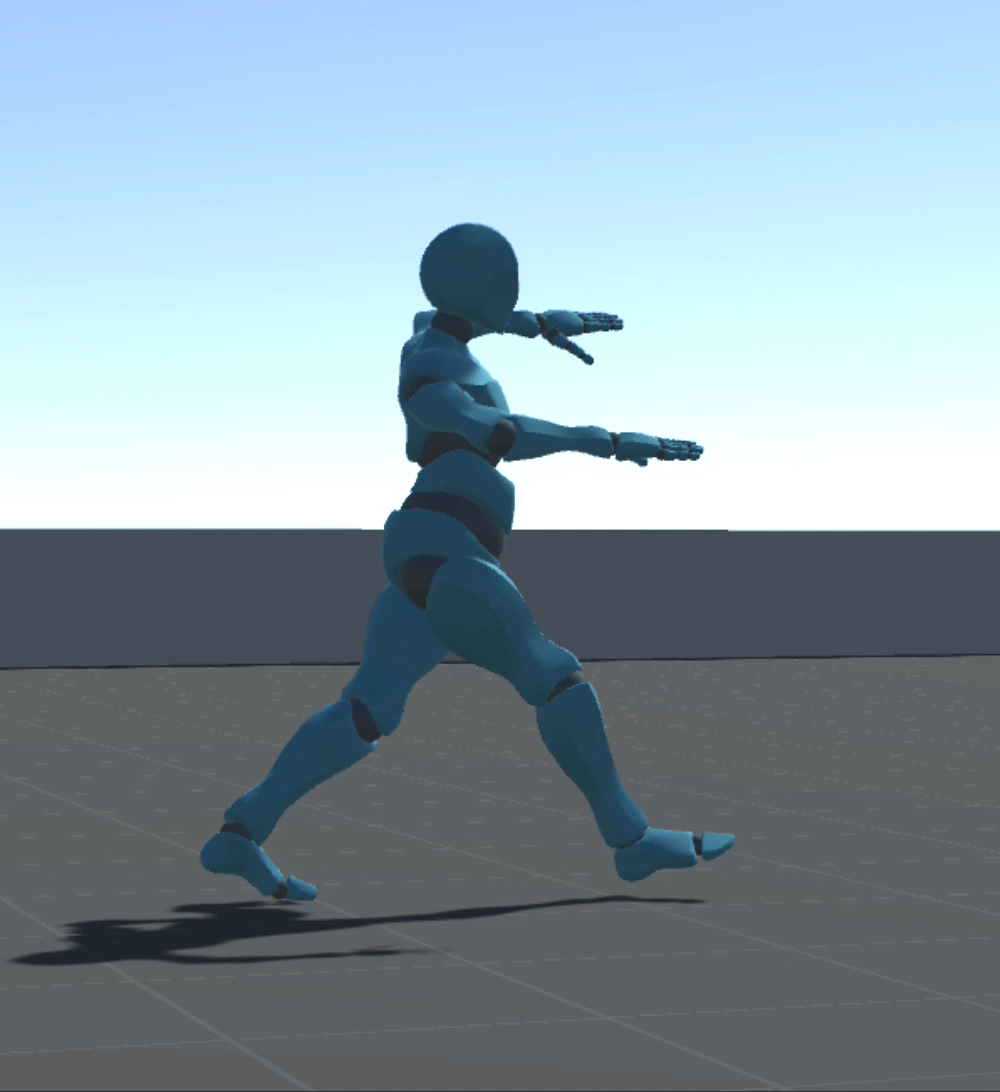
\includegraphics[width=0.27\textwidth]{img/charakter_mixamo_laufen6} \\
  \end{tabular}
  \caption{Mixamo Versuch 11 Gangbild}
  \label{fig:mixamo_versuch11_gangbild}
\end{figure}

\subsection{Belohnung für Energieminimierung}
Ein großer Einfluss auf die Entwicklung des menschlichen Gangbilds ist die Energieminimierung. Der Läufer hat keine Wahrnehmung von Aufwand, daher sind die erlernten Bewegungsabläufe oft alles andere als effizient. Um das Gangbild weiter zu verbessern wird eine Belohnung eingeführt welche den Agenten belohnt wenn er so wenig wie möglich Kraft aufwendet um das Ziel zu erreichen. Genauer gesagt wird er dafür bestraft wenn die Gelenksteuerung einen zu hohe Energiekonsum aufweist. Ähnlich wie die Fußwechselbestrafung wird auch für die Energieminimerung eine Funktion verwendet welche die Bestrafung zwischen 150 und 3150 Watt linear ansteigt.

\begin{figure}[H]
  \centering
  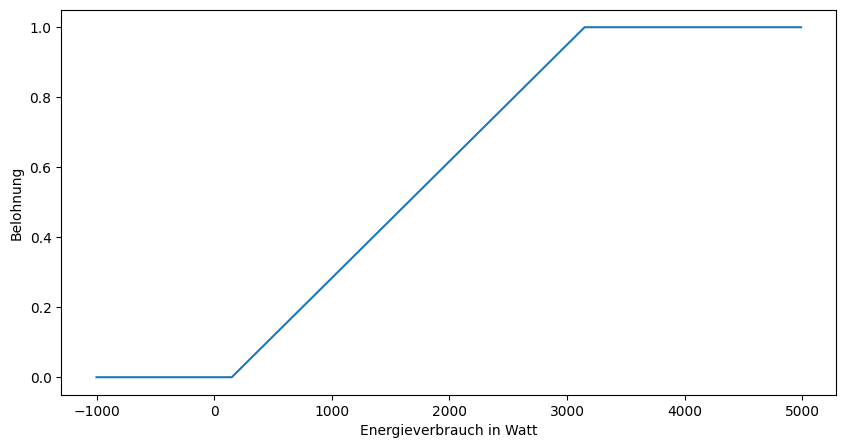
\includegraphics[width=0.9\textwidth]{img/plot_energiespar} 
  \caption{Energiespar Belohnung}
  \label{fig:plot_energiespar}
\end{figure}

Die Energieminimierung bringt den Läufer dazu seine Bewegungen zu optimieren und somit zu minimieren. Das Gangbild wirkt dadurch natürlicher. Vor allem die Bein und Körperbewegungen wurden wesentlich verbessert. Die Arme werden so gut wie gar nicht mehr bewegt um so viel Energie wie möglich zu sparen.

\begin{figure}[H]
  \centering
  \begin{tabular}{ccc}
    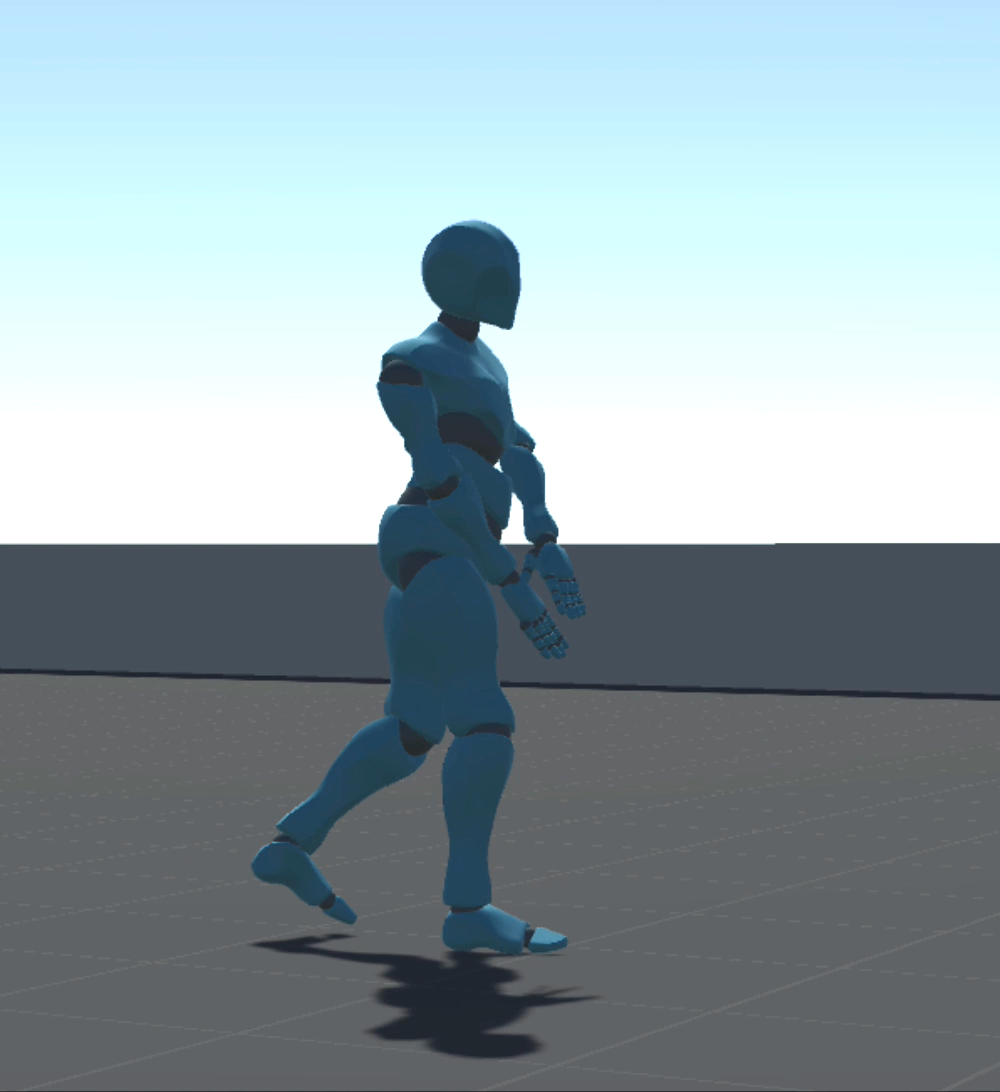
\includegraphics[width=0.27\textwidth]{img/charakter_mixamo_laufen_energiespar1} & 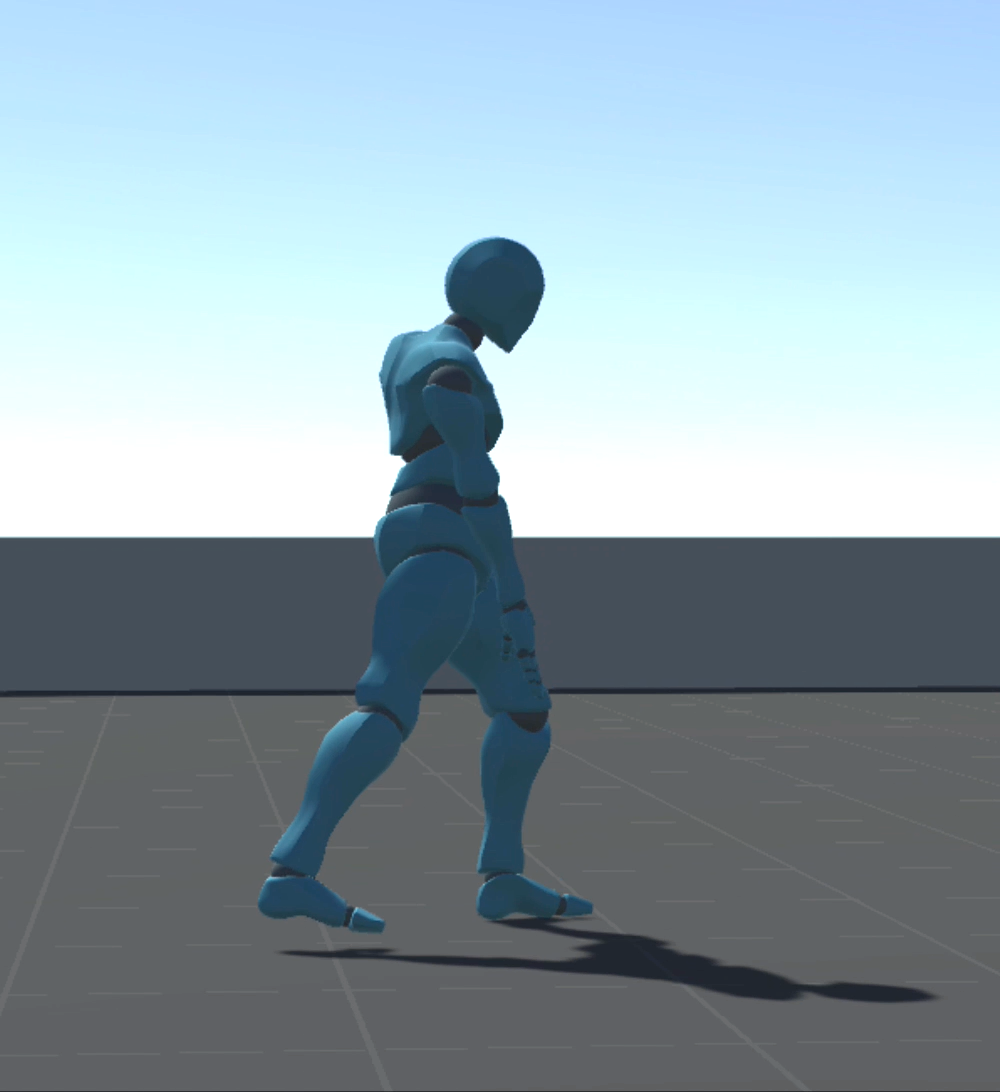
\includegraphics[width=0.27\textwidth]{img/charakter_mixamo_laufen_energiespar2}  & 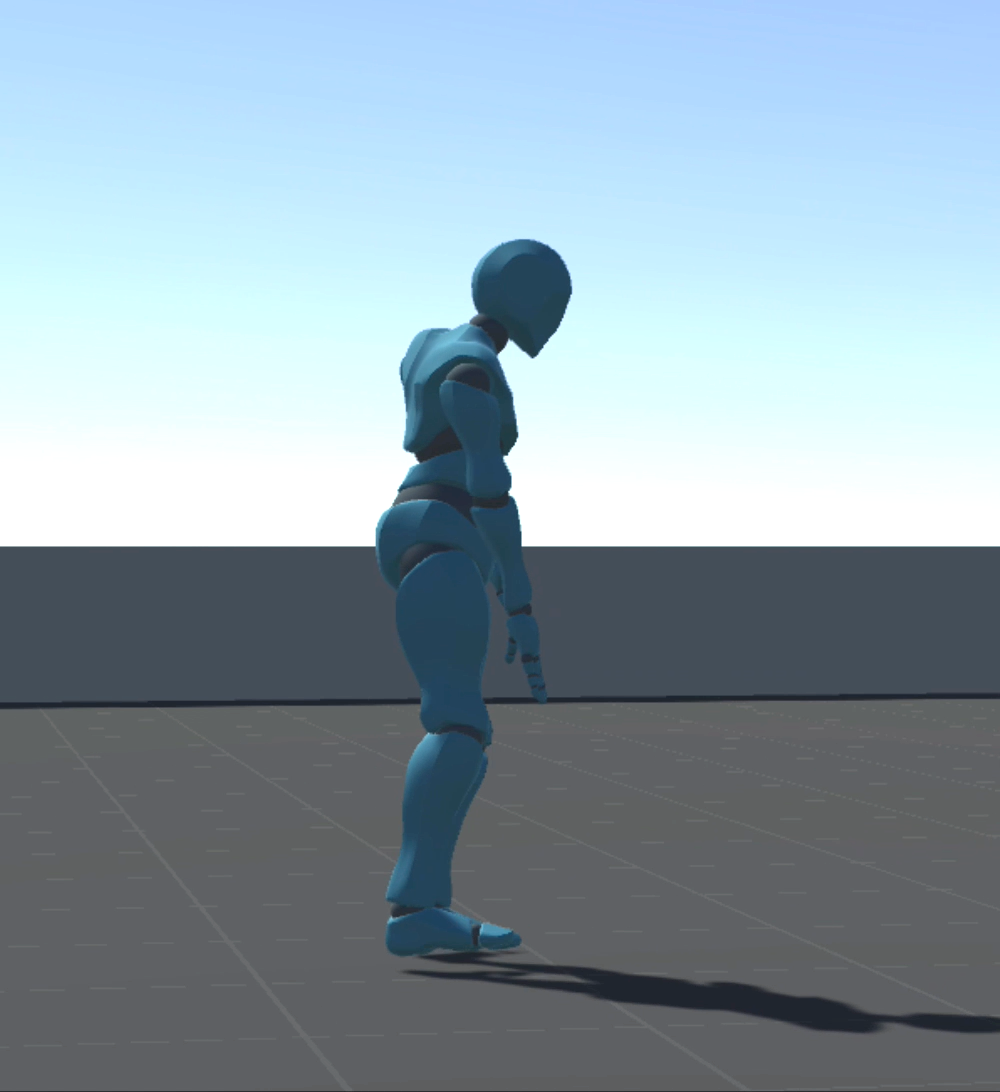
\includegraphics[width=0.27\textwidth]{img/charakter_mixamo_laufen_energiespar3} \\
    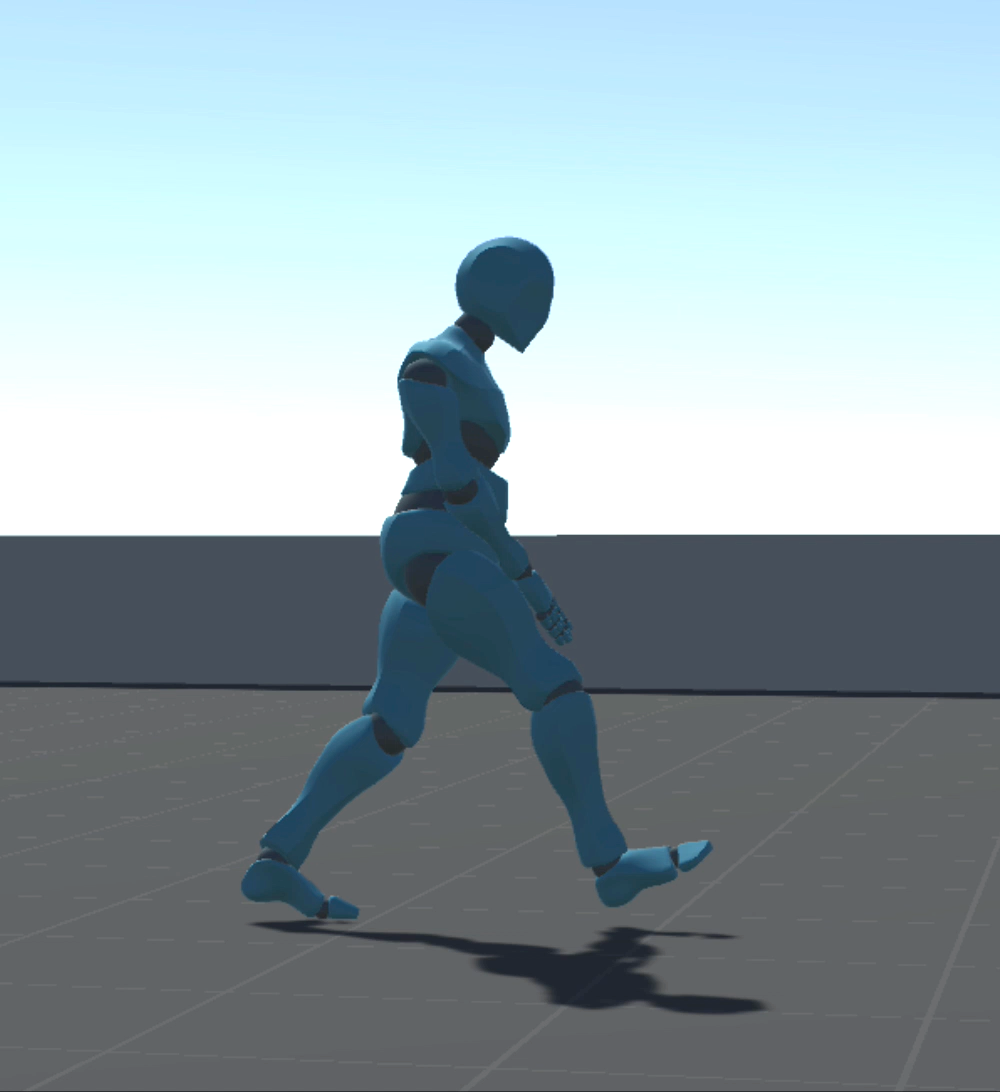
\includegraphics[width=0.27\textwidth]{img/charakter_mixamo_laufen_energiespar4}  & 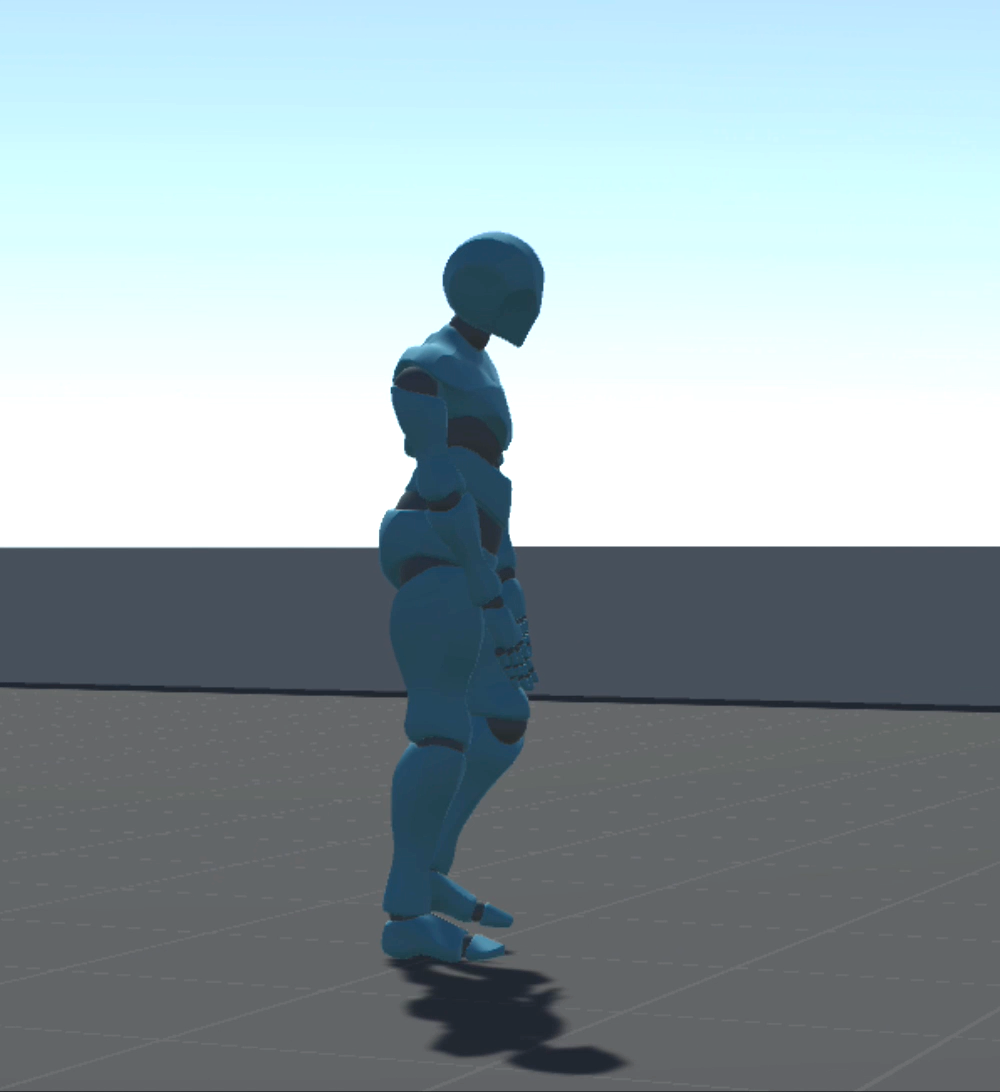
\includegraphics[width=0.27\textwidth]{img/charakter_mixamo_laufen_energiespar5}  & 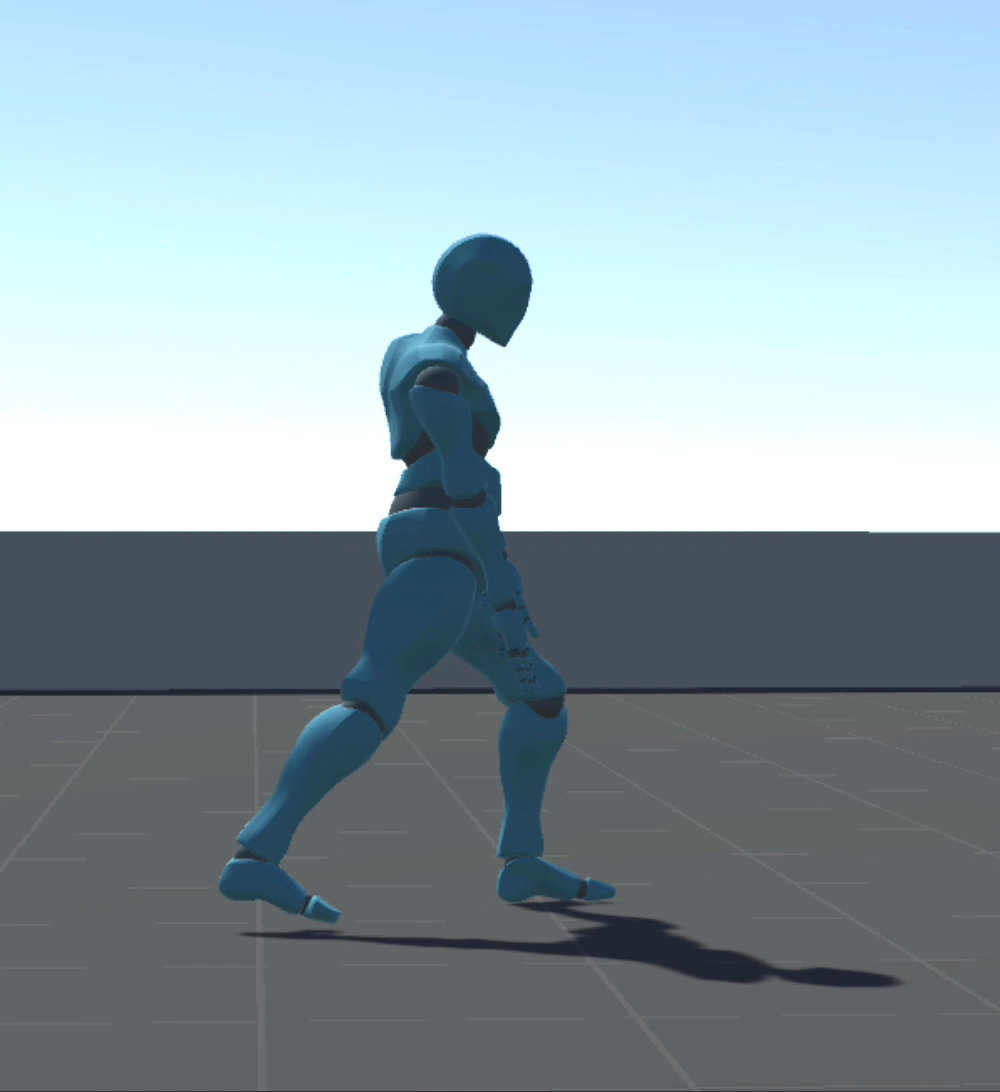
\includegraphics[width=0.27\textwidth]{img/charakter_mixamo_laufen_energiespar6} \\
  \end{tabular}
  \caption{Mixamo Versuch 12 Gangbild}
  \label{fig:mixamo_versuch12_gangbild}
\end{figure}

\subsection{Belohnung Armpendel}
Die Arme sind für eine natürliche Gehbewegung unabdinglich. Ein gesunder Mensch bewegt die Arme beim gehen gegensätzlich zu den Beinen. Einige Vermutungen warum der Mensch dieses Verhalten zeigt sind die Verbesserung der Stabilität, Energieminimierung oder die Abstammung von Vorfahren welche die Arme aktiv beim fortbewegen einsetzten.\cite{meyns2013and}

Der Grund ist für die Entwicklung eines natürlichen Charakterkontrollers jedoch zweitrangig. Durch die vereinfachte physikalische Darstellung muss das für Menschen natürliche Verhalten teilweise über Umwege antrainiert werden.

\subsection{Imitationslernen}